\documentclass[border=5pt]{standalone}
\usepackage{tikz}
\usetikzlibrary{bayesnet}
\begin{document}
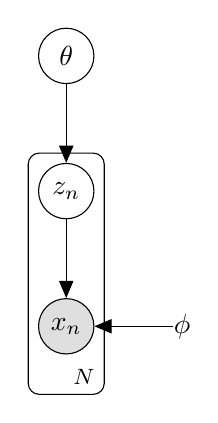
\begin{tikzpicture}
\node[latent] (theta) {$\theta$};
\node[latent, below=of theta] (z) {$z_n$};
\node[obs, below=of z] (x) {$x_n$};
\node[const, right=of x] (phi) {$\phi$};
\edge {theta} {z};
\edge {z, phi} {x};
\plate {plate} {(z)(x)} {$N$};
\end{tikzpicture}
\end{document}
